\documentclass{article}
\usepackage[utf8]{inputenc}
\usepackage{graphicx}
\usepackage{enumitem}
\usepackage{siunitx}
\usepackage{multirow}
\usepackage[a4paper, total={6in, 8in}]{geometry}
\usepackage[style=authoryear-ibid,backend=biber]{biblatex}
\usepackage[swedish]{babel}
\usepackage{float}
\usepackage{caption}
\usepackage[parfill]{parskip}
\usepackage{amsmath}
\usepackage{csquotes}
\usepackage{comment}
\usepackage{url}


\graphicspath{ {img/} }

\title{\Huge Operating Systems - Study \\ EDAF35}
%\author{\Large Elias Bergström, Emma Lindh, Elin Helmersson, Shahriar Chegini}
\author{  
    Elias Bergström\\
    \texttt{el8025be-s@student.lu.se}
    }
%\date{VT2024}
\date{\today}

\renewcommand{\figurename}{Figur}
\renewcommand{\tablename}{Tabell}

%handledarens namn

\begin{document}

\maketitle
\thispagestyle{empty}
%\pagenumbering{gobble}
\pagebreak
%\thispagestyle{empty}
%\pagenumbering{arabic}

\section{Module 1}

\subsection{Red Box!}
\begin{itemize}
    \item User mode and kernel mode are important concepts!
    (Section 1.4.2 in Operating System Concepts)
    \item Handling a system call. (Covered in section 2.3.2 in Operating System Concepts)
    \item OS structures, important to understand the different structures (monolithic, layered, microkernels, modules and hybrid systems) and their trade-offs. Covered in section 2.8 in Operating System Concepts.
\end{itemize}

\subsection{User and Kernel mode}

\paragraph{What are User Mode and Kernel Mode?}
User mode and kernel mode are two distinct execution modes in a computer system that separate the level of privilege and access to system resources. This separation ensures system stability and security.

\begin{itemize}
    \item \textbf{User Mode:}
    \begin{itemize}
        \item The mode in which user applications run.
        \item Access to system resources and hardware is restricted.
        \item System calls must be used to request services from the operating system.
    \end{itemize}
    
    \item \textbf{Kernel Mode:}
    \begin{itemize}
        \item The mode in which the operating system runs.
        \item Full access to all system resources, including hardware and memory.
        \item Executes critical tasks like process management, memory management, and device handling.
    \end{itemize}
\end{itemize}

\paragraph{Why are User Mode and Kernel Mode Important?}
\begin{itemize}
    \item They ensure system stability by preventing user applications from directly accessing or modifying critical system resources.
    \item They enhance security by isolating user applications from the operating system kernel.
    \item They enable efficient multitasking and resource management by allowing the operating system to control access to hardware and shared resources.
\end{itemize}





\subsection{System Call}


\paragraph{What is a System Call?}
A system call is a mechanism used by user-level applications to request services from the operating system's kernel. These services include operations like file manipulation, process management, and memory allocation.

\paragraph{Steps in Handling a System Call:}
\begin{enumerate}
    \item \textbf{Triggering the System Call:}
    \begin{itemize}
        \item The user application invokes a system call, typically through a library function.
        \item A special CPU instruction, such as \texttt{INT} (Interrupt) or \texttt{SYSENTER}, switches the execution mode from user mode to kernel mode.
    \end{itemize}
    
    \item \textbf{Identifying the System Call:}
    \begin{itemize}
        \item The system call number is passed to the kernel, usually via a specific register or stack.
        \item The kernel uses this number to determine the requested service.
    \end{itemize}
    
    \item \textbf{Processing the Request:}
    \begin{itemize}
        \item The kernel executes the corresponding system call handler.
        \item This may involve interacting with hardware, managing resources, or performing calculations.
    \end{itemize}
    
    \item \textbf{Returning to User Mode:}
    \begin{itemize}
        \item The kernel completes the system call and prepares the return value or status.
        \item The CPU switches back to user mode, and the control returns to the user application.
    \end{itemize}
\end{enumerate}

\paragraph{Example:}
For a \texttt{read()} system call:
\begin{itemize}
    \item The application calls \texttt{read()}, specifying the file descriptor, buffer, and size.
    \item The kernel checks permissions, retrieves the data from the file, and writes it to the buffer.
    \item The system call returns the number of bytes read or an error code.
\end{itemize}


\begin{figure}[H]
    \centering
    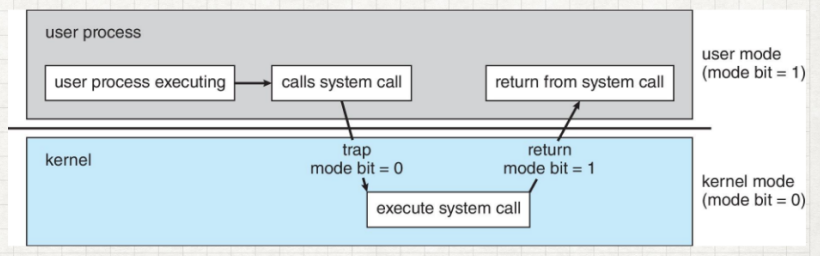
\includegraphics[width=0.8\textwidth]{syscall.png}
    \caption{Diagram of a system call.}
    \label{fig:syscall}
\end{figure}


\subsection{OS Structures}

\paragraph{Monolithic Structure}
\begin{itemize}
    \item \textbf{Description:} All OS components are contained in a single, large kernel.
    \item \textbf{Advantages:}
    \begin{itemize}
        \item High performance due to minimal communication overhead.
        \item Simple to implement and efficient for tightly coupled systems.
    \end{itemize}
    \item \textbf{Disadvantages:}
    \begin{itemize}
        \item Difficult to maintain and debug due to lack of modularity.
        \item A single failure can compromise the entire system.
    \end{itemize}
\end{itemize}

\paragraph{Layered Structure}
\begin{itemize}
    \item \textbf{Description:} OS is divided into layers, each built on top of the other, with clear interfaces.
    \item \textbf{Advantages:}
    \begin{itemize}
        \item Easier to maintain and extend due to modular design.
        \item Improves security and stability by isolating functionalities.
    \end{itemize}
    \item \textbf{Disadvantages:}
    \begin{itemize}
        \item Overhead from inter-layer communication.
        \item Can be less efficient due to strict layering.
    \end{itemize}
\end{itemize}

\paragraph{Microkernels}
\begin{itemize}
    \item \textbf{Description:} Minimal kernel providing core functions like communication and basic scheduling, with other services running in user space.
    \item \textbf{Advantages:}
    \begin{itemize}
        \item Highly modular and easier to extend or modify.
        \item Improved security and reliability since most services run in user mode.
    \end{itemize}
    \item \textbf{Disadvantages:}
    \begin{itemize}
        \item Higher communication overhead between user space and kernel.
        \item Slower performance compared to monolithic kernels.
    \end{itemize}
\end{itemize}

\paragraph{Modules}
\begin{itemize}
    \item \textbf{Description:} The OS kernel is extensible via loadable modules, which can be dynamically added or removed. This type of design is common in modern implementations
    of UNIX , such as Linux, macOS, and Solaris, as well as Windows. 
    \item \textbf{Advantages:}
    \begin{itemize}
        \item Combines the efficiency of monolithic kernels with the flexibility of modularity.
        \item Reduces the kernel size by loading only necessary modules.
    \end{itemize}
    \item \textbf{Disadvantages:}
    \begin{itemize}
        \item Compatibility issues may arise between modules.
        \item Bugs in modules can still compromise the kernel.
    \end{itemize}
\end{itemize}

\paragraph{Hybrid Systems}
\begin{itemize}
    \item \textbf{Description:} A combination of microkernel and monolithic design, incorporating the benefits of both.
    \item \textbf{Advantages:}
    \begin{itemize}
        \item Balances performance and modularity.
        \item Adaptable to various system requirements.
    \end{itemize}
    \item \textbf{Disadvantages:}
    \begin{itemize}
        \item Increased complexity in design and implementation.
        \item May not fully exploit the advantages of either microkernels or monolithic kernels.
    \end{itemize}
\end{itemize}

\pagebreak


\section{Module 2 - Processes and Threads}
\subsection{Red Box}
\begin{itemize}
    \item It is important to understand what the PCB is and that the PCBs get put on different queues by the OS when
    managing process state.
    (From section 3.1.3 to the end of 3.2.1 in Operating System Concepts)
    \item You need to understand process creation (including fork() and exec() in detail) and process termination (including
    zombie and orphan processes). From section 3.1.3 to the end of 3.2.1 in Operating System Concepts)
    \item You need to understand the difference between user threads and kernel threads and the different models for
    mapping between the two (Section 4.3 in Operating System Concepts)
\end{itemize}

\subsection{Notes}



The process can be in a number of different states, see figure.

\begin{figure}[H]
    \centering
    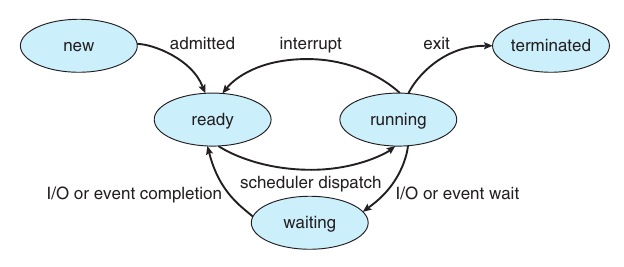
\includegraphics[width=0.8\textwidth]{pcb.png}
    \caption{Diagram of process states}
    \label{fig:diapcb}
\end{figure}


\subsubsection{PCB}
PCB stands for Process Control Block and each process is represented in the OS by one. The PCB contains information about the process:
\begin{itemize}
    \item {\bf Process state.} The state may be new, ready, running, waiting, halted, and
    so on.
    \item {\bf Program counter.} The counter indicates the address of the next instruction
    to be executed for this process.
    \item {\bf CPU registers.}
    \item {\bf CPU-scheduling information.} This information includes a process prior-
    ity, pointers to scheduling queues, and any other scheduling parameters.
    (Chapter 5 describes process scheduling.)
    \item {\bf Memory-management information.} This information may include such
    items as the value of the base and limit registers and the page tables, or the
    segment tables, depending on the memory system used by the operating
    system (Chapter 9).
    \item {\bf Accounting information} This information includes the amount of CPU
    and real time used, time limits, account numbers, job or process numbers,
    and so on.
    \item {\bf I/O status information.} This information includes the list of I/O devices
    allocated to the process, a list of open files, and so on.
\end{itemize}
In brief, the PCB simply serves as the repository for all the data needed to start,
or restart, a process, along with some accounting data.

\subsection*{fork() and exec() in Unix/Linux Context}

In a Unix/Linux context, \texttt{fork()} and \texttt{exec()} are system calls used for process creation and management.

\subsubsection*{fork()}
The \texttt{fork()} system call creates a new process by duplicating the calling (parent) process. The new process is called the \textit{child} process. Both the parent and the child process continue executing from the point of the \texttt{fork()} call. The child process gets a copy of the parent’s memory space, but they have different Process IDs (PIDs). \texttt{fork()} returns:
\begin{itemize}
    \item \texttt{0} in the child process.
    \item The child’s PID in the parent process.
\end{itemize}

\subsubsection*{exec()}
The \texttt{exec()} family of functions (e.g., \texttt{execvp()}, \texttt{execp()}, etc.) replaces the current process’s memory space with a new program. After calling \texttt{exec()}, the process image is completely replaced, and the new program starts executing. This is commonly used after \texttt{fork()} when the child process needs to run a different program than the parent.

\subsubsection*{Typical Usage}
In typical usage:
\begin{enumerate}
    \item \texttt{fork()} is used to create a new process.
    \item \texttt{exec()} is used by the child (or parent) to replace its process image with a different program.
\end{enumerate}

Together, these calls enable the creation of new processes and the execution of different programs, which is fundamental for tasks like launching new applications or running shell commands.



\subsubsection{Multithreading Models}
These models describes how to map user thread to kernel threads. User threads are supported above the kernel and are managed without kernel support and the kernel threads are managed by the kernel.

\begin{itemize}
    \item {\bf Many-to-One Model}, all user threads are mapped to one kernel 
    thread, where the switching between threads are done by a thread library in user space (not by the kernel)
    It's efficient but if the current user threads hangs it will also hang the kernel thread.
    \item {\bf One-to-One Model}, maps each user thread to a kernel thread. Multiple threads can run at the same time. The problem with this model is that you need to create a kernel thread for each user thread.
    \item {\bf Many-to-Many}, multiplexs many user threads to a smaller or equal amount of kernel threads.
    \item {\bf Two-Level Model} mixing two of the models. 
\end{itemize}




\section{Module 3.A - CPU Scheduling}
\subsection{Red Box}
\begin{itemize}
    \item Make sure you understand what it means for scheduling to be pre-emptive.
    (From section 5.1.3 in Operating System Concepts)
    \item You need to know and understand the tradeoffs between these different algorithms
    (Section 5.3 in Operating System Concepts)
    \item Be able to understand the differences between process and system contention scopes
    (Section 5.4 in Operating System Concepts)
    \item You need to understand ready queues, load balancing and processor affinity in multiprocessor systems
    (Section 5.5.1, 5.5.3 and 5.5.4 ins Operating System Concepts)
    \item You need to understand what makes real time scheduling different, the periodic process model and the
    differences between the RMS and the EDF scheduler (Section 5.6.1 – 5.6.4 in Operating System Concepts)
\end{itemize}

\begin{enumerate}
    \item When a process switches from the running state to the waiting state (for
    example, as the result of an I/O request or an invocation of wait() for the
    termination of a child process)
    \item When a process switches from the running state to the ready state (for
    example, when an interrupt occurs)
    \item When a process switches from the waiting state to the ready state (for
    example, at completion of I/O)
    \item When a process terminates
\end{enumerate}

When scheduling takes place only under circumstances 1 and 4, we say that the scheduling scheme is non preemptive or cooperative.
Otherwise, it is {\bf preemptive}. 
\\
\\
Chatgpt says the following:
\\ {\it Preemptive scheduling is a CPU scheduling method where the operating system can interrupt a running process to give the CPU to another process, usually with higher priority or urgency.
In this system, the OS can stop a process and switch to another one, either after a fixed time slice (in round-robin scheduling) or if a higher-priority process needs the CPU.}

\subsection{Scheduling Algorithms}

\subsubsection{First-Come, First-Served Scheduling (FCFS)}
This is the simplest algorithm. With this scheme, the process that requests the
CPU first is allocated the CPU first. The implementation of the FCFS policy is
easily managed with a FIFO queue. When a process enters the ready queue, its
PCB is linked onto the tail of the queue. When the CPU is free, it is allocated to
the process at the head of the queue. The running process is then removed from
the queue. The code for FCFS scheduling is simple to write and understand.
On the negative side, the average waiting time under the FCFS policy is
often quite long. {\bf Pro: simplest Con: Can have long wait times}.

\subsubsection{Shortest-Job-First (SJF) Scheduling}
Do the shortest job first. If to jobs take the same time FCFS is used to break the tie.
The more appropriate term for this method is {\bf shortest-next-CPU-burst}, because scheduling depends on the length of the next CPU burst of
a process, rather than its total length. 


Although the SJF lagorithm is optimal, it cannot be implemented at the level of CPU scheduling, 
as there is no way to know the length of the next CPU burst.
One approach to this problem is to try to approximate SJF scheduling. We may
not know the length of the next CPU burst, but we may be able to predict its
value. We expect that the next CPU burst will be similar in length to the previous
ones. By computing an approximation of the length of the next CPU burst, we
can pick the process with the shortest predicted CPU burst.


{\bf Pro: less down time then FCFS Con: harder to implement.}

 
{\bf Whats the difference between Job and CPU burst?}


\subsubsection{Round-Robin (RR) Scheduling}

Similar to FCFS but with preemption added. 

To implement RR scheduling, we again treat the ready queue as a FIFO
queue of processes. New processes are added to the tail of the ready queue.
\\
The CPU scheduler picks the first process from the ready queue, sets a timer to
interrupt after 1 time quantum, and dispatches the process.
One of two things will then happen. The process may have a CPU burst of
less than 1 time quantum. In this case, the process itself will release the CPU
voluntarily. The scheduler will then proceed to the next process in the ready
queue. If the CPU burst of the currently running process is longer than 1 time
quantum, the timer will go off and will cause an interrupt to the operating
system. A context switch will be executed, and the process will be put at the
tail of the ready queue. The CPU scheduler will then select the next process in
the ready queue.
\\

{\bf Con: the average waiting time under RR is often long. Pro: Relatively simple.}


\subsubsection{Priority Scheduling}

SJF is a special case of the general priority-scheduling. 
\\
A priority is associated with each process, and the CPU is allocated to the process with the highest priority. Equal-priority processes are scheduled in
FCFS order. An SJF algorithm is simply a priority algorithm where the priority
(p) is the inverse of the (predicted) next CPU burst. The larger the CPU burst,
the lower the priority, and vice versa.
\\


{\bf Con: different systems have different levels of priority, i.e. code is not portable.}



\subsubsection{Multilevel Queue Scheduling}

Separate queues for different priority levels. Often use RR per queue.
\\
{\bf Pro: you don't need to do an O(n) search to find the task with the highest priority.}



\subsubsection{Multilevel Feedback Queue Scheduling}

It's the same as Multilevel Queue Scheduling, but tasks can move between queues. 



\subsection{Differences between process and system contention scopes.} %page 217

Process contention scope and system contention scope are two types of thread scheduling models used to determine 
how threads compete for CPU time. They define the level at which threads contend for CPU 
resources, either within a process or across the entire system.



\subsubsection{Process Contention Scope (PCS)}

\begin{itemize}
    \item {\bf Scope:} Threads within the same process contend for CPU time only with other threads of that same process.
    \item {\bf Scheduling:} Threads are scheduled based on the process's thread priority and its own internal scheduling policies. The OS doesn't consider other processes' threads when scheduling threads for a particular process.
    \item {\bf Example:}Example: If two threads are running in a single process, they compete for CPU time only with each other, without interference from threads of other processes.
\end{itemize}


\subsubsection{System Contention Scope (SCS)}

\begin{itemize}
    \item {\bf Scope:} Threads from all processes in the system compete for CPU time against each other, regardless of the process they belong to.
    \item {\bf Scheduling:} Threads are scheduled system-wide, with the OS considering all threads in the system, not just those within the same process.
    \item {\bf Example:} Threads from different processes (e.g., Thread A from Process 1 and Thread B from Process 2) compete for CPU time on the same level, meaning the OS schedules them based on their priority relative to each other.
\end{itemize}

In short, {\bf PCS} is more localized within a process, while {\bf SCS} involves all threads in the system competing for CPU time.





\section{Module 3.B - Synchronization}
\subsection{Red Box}
\begin{itemize}
    \item You should know what the critical section problem is (Section 6.2 in Operating System Concepts)
    \item You must know the differences between Spinlocks, Semaphores and Mutexes in the context of Operating
    (Systems. 6.5 and 6.6 in Operating System Concepts – not the clearest explanation. Chapter 9, 10 in Linux Kernel
    development )
\end{itemize}



\subsection{Critical Section Problem}

The critical-section problem is to design a protocol that the processes can use to 
synchronize their activity so as to cooperatively share data. I.E, when one process is executing in it's
critical section another process can't do the same.
\\
A solution to this problem must satisfy the following:

\begin{enumerate}
    \item {\bf Mutual exclusion.} If a process is executing in its critical section, then no
    other processes can be executing in their critical sections.
    \item {\bf Progress.} If no process is executing in its critical section and some pro-
    cesses wish to enter their critical sections, then only those processes that
    are not executing in their remainder sections can participate in deciding which 
    will enter its critical section next, and this selection cannot be
    postponed indefinitely.
    \item {\bf Bounded waiting.} There exists a bound, or limit, on the number of times
    that other processes are allowed to enter their critical sections after a
    process has made a request to enter its critical section and before that
    request is granted.
\end{enumerate}


%You must know the differences between Spinlocks, Semaphores and Mutexes in the context of Operating

\subsection{Different types of locks}

\begin{itemize}
    \item {\bf Mutexes.} A mutex (mutual exclusion) lock is a synchronization mechanism that ensures only one thread can 
    access a shared resource at a time, preventing race conditions. 
    When a thread locks the mutex, others must wait until it is released, 
    ensuring exclusive access and data integrity during concurrent operations.
    \item {\bf Spinlocks.} A type of mutex lock where the process "spins" (busy-waits) for acquire. 
    \item {\bf Semaphores.} A integer var that is access through two atomic operations: wait() and signal().
\end{itemize}





\section{Module 4 - Memory Management}
\subsection{Red Box}
\begin{itemize}
    \item You need to understand what the physical and logic address space is and the motivation behind it. You also need to understand that
    the mmu is required to translate between the two (9.1.1 to 9.1.4 in operating system concepts).
    \item You need to understand what contigous allocation is, how it works and why fragmentation is a major issue.
    (section 9.2 in operating system concepts)
    \item You need to understand what paging is, what the page table and tlb are,
    and have a general idea of what protection and shared
    pages are (section 9.2 in operating system concepts).
    \item You need to know why we cannot use simple page tables, the three alternative page table structures and the advantages and
    disadvantages of each (section 9.4 of operating system concepts).
    \item You need to understand the basic concepts of virtual memory and its advantages(section 10.1 of operating system concepts).
    \item You need to be able to explain what demand paging is, free frame list and its performance (section 10.2 of operating system concepts).
    \item You need to know what page replacement is, understand the main three different page replacement algorithms discussed in the book
    and their tradeoffs, and be able to describe belady’s anomaly (section 10.4 of operating system concepts).
\end{itemize}


\subsection{Physical and logic address space and MMU}

The physical address space refers to the actual addresses in the RAM (hardware memory), 
while the logical address space refers to the addresses used by programs during execution, 
which are mapped to physical addresses by the operating system.
\newline

{\bf Key differences:}
\begin{itemize}
    \item {\bf Physical Address:} Actual memory locations in RAM.
    \item {\bf Logical Address:} Virtual addresses used by programs.
    \item {\bf Mapping: } Logical addresses are mapped to physical addresses by the MMU.
\end{itemize}

{\bf Reason:}
\begin{itemize}
    \item {\bf Isolation \& Protection:} Logical addresses allow programs to operate in isolated, virtualized memory spaces, preventing interference between programs.
    \item {\bf Efficient Memory Use:} Virtual memory lets programs use more memory than physically available by swapping data between RAM and disk storage.
\end{itemize}

The MMU (Memory Management Unit) is a hardware component in a computer that manages memory operations,
specifically the mapping between logical addresses (used by programs) and physical addresses
(actual memory locations in RAM).

\subsection{Contigous Allocation}

Contiguous allocation is a memory management method where each process is assigned a single, 
continuous block of memory. 
It works by allocating a process a large enough, uninterrupted segment of RAM.

{\bf Fragmentation}
\begin{itemize}
    \item {\bf External Fragmentation:} Free memory is scattered in small blocks, making it hard to allocate large blocks even though there’s enough total free memory.
    \item {\bf Internal Fragmentation:} Allocated memory is larger than needed, wasting space within the block.
\end{itemize}
Fragmentation leads to wasted memory, inefficient use of available space, and can cause allocation failures, reducing system performance.

\subsection{Paging, Page Table and TLB (Translation Lookaside Buffer)}
{\bf Paging} is a memory management technique that divides the virtual address space and physical memory into fixed-size blocks called pages (virtual memory) and frames (physical memory). Virtual addresses are translated to physical addresses through a page table.
\newline
\newline
The {\bf page table} is a data structure that maps virtual page numbers to physical frame numbers. It includes additional information like access permissions and whether the page is in memory.
\newline
\newline
The {\bf TLB} is a small, fast cache that stores recently used page table entries. It speeds up address translation by reducing the need to access the page table repeatedly. A TLB hit avoids a slower lookup, while a TLB miss requires accessing the page table.

\subsection{Protected and Shared Pages}

{\bf Protected Pages: } Memory pages with restricted access to prevent unauthorized operations (e.g., writing to read-only pages). Enforced through page table permissions to ensure process isolation and security.
\newline
\newline
{\bf Shared Pages: } Memory pages accessible by multiple processes, allowing shared libraries or interprocess communication. Each process's page table maps to the same physical memory frame.

\subsection{Simple Page Tables}

\paragraph{Why They Are Not Feasible}
Simple page tables are impractical for systems with large virtual address spaces due to:

\begin{itemize}
    \item \textbf{High Memory Overhead:} A page table must have one entry per virtual page. For large address spaces, this requires enormous memory.
    \item \textbf{Inefficiency for Sparse Usage:} Many processes use only a small portion of their address space, leading to wasted memory.
    \item \textbf{Scalability Issues:} Large page tables are difficult to manage and update, especially with multiple processes.
    \item \textbf{Performance Impact:} Large tables increase latency in address translation and are harder to cache in the TLB.
\end{itemize}

\subsection{Three alternative page table structures}

\subsubsection{Hierarchical Paging}
Hierarchical paging is a method of managing large page tables by dividing them into smaller, more manageable parts using multiple levels. This approach reduces memory usage for page tables and handles sparsely populated address spaces efficiently.

{\bf How it works:}
\begin{enumerate}
    \item {\bf structure}
    \begin{itemize}
        \item The page table is split into multiple levels (e.g., two-level, three-level).
        \item The virtual address is divided into sections, each corresponding to a level in the hierarchy.
    \end{itemize}
    \item Translation Steps:
    \begin{itemize}
        \item The virtual address is divided into: \begin{itemize}
            \item Page directory index: Points to the page directory.
            \item Page table index: Points to the specific page table.
            \item Offset: Specifies the exact location within the page.
        \end{itemize}
    \item The CPU first accesses the page directory to locate the relevant page table.
    \item Then, it accesses the specific page table to find the physical frame.
    \end{itemize}
\end{enumerate}

{\bf Advantages:}
\begin{itemize}
    \item Saves memory by only allocating page tables for used address spaces.
    \item Efficient for sparse virtual memory systems.
\end{itemize}

{\bf Example for a two-level system:} 
\\
A 32-bit address might be divided as: 
\begin{itemize}
    \item 10 bits for the page directory,
    \item 10 bits for the page table,
    \item 12 bits for the offset within a page.
    This structure allows addressing large memory while keeping page tables compact.
\end{itemize}

\subsubsection{Hashed Page Tables}

Hashed page tables are a memory management scheme designed for systems with large address spaces. Instead of using a hierarchical structure, they utilize a hash table to efficiently map virtual addresses to physical frames.

\paragraph{How It Works}
\begin{enumerate}
    \item \textbf{Hash Function:}
    \begin{itemize}
        \item A hash function computes an index from the virtual page number.
        \item This index points to a linked list (or bucket) of entries in the hash table.
    \end{itemize}

    \item \textbf{Entries:}
    \begin{itemize}
        \item Each entry contains:
        \begin{itemize}
            \item Virtual page number.
            \item Corresponding physical frame number.
            \item A pointer to the next entry (in case of collisions).
        \end{itemize}
    \end{itemize}

    \item \textbf{Translation:}
    \begin{itemize}
        \item When a process needs to access memory, the virtual page number is hashed.
        \item The system searches the bucket for a matching entry.
        \item If found, the physical frame number is retrieved, and the memory is accessed.
    \end{itemize}
\end{enumerate}

\paragraph{Advantages}
\begin{itemize}
    \item Efficient for large and sparse address spaces.
    \item Reduces the memory overhead of traditional page tables.
\end{itemize}

\paragraph{Disadvantages}
\begin{itemize}
    \item Slower in the case of hash collisions, as it requires traversing a linked list.
    \item Slightly more complex than simple or hierarchical page tables.
\end{itemize}

\subsubsection{Inverted Page Tables}

Inverted page tables are a memory management technique used to reduce the memory overhead of traditional page tables by storing a single global page table for the entire system, rather than one table per process.

\paragraph{How It Works}
\begin{enumerate}
    \item \textbf{Structure:}
    \begin{itemize}
        \item Each entry in the inverted page table corresponds to a physical frame in memory.
        \item Entries contain:
        \begin{itemize}
            \item Virtual page number.
            \item Process ID (to identify which process owns the page).
            \item Control bits (e.g., valid, protection).
        \end{itemize}
    \end{itemize}

    \item \textbf{Translation:}
    \begin{itemize}
        \item When a virtual address needs to be translated:
        \begin{enumerate}
            \item The system searches the inverted page table for an entry matching the virtual page number and process ID.
            \item If a match is found, the corresponding physical frame number is used to access memory.
            \item If no match is found, a page fault occurs.
        \end{enumerate}
    \end{itemize}
\end{enumerate}

\paragraph{Advantages}
\begin{itemize}
    \item Significantly reduces memory usage by having a single global page table.
    \item Efficient for systems with large address spaces.
\end{itemize}

\paragraph{Disadvantages}
\begin{itemize}
    \item Slower lookups due to the need for searching the entire table (typically mitigated using hashing).
    \item More complex compared to traditional page tables.
\end{itemize}

\subsection{Virtual Memory}

Virtual memory is a technique that allows processes to use more memory than physically available by using disk storage as an extension of RAM. 

\paragraph{Advantages}
\begin{itemize}
    \item Provides process isolation and memory protection.
    \item Enables efficient utilization of physical memory.
    \item Supports large address spaces, allowing programs to run regardless of physical memory size.
    \item Facilitates multiprogramming by allowing multiple processes to share memory safely.
\end{itemize}

\subsection{Demand Paging and Free Frame List}

\paragraph{Demand Paging}
Demand paging is a technique where pages are loaded into memory only when they are needed, rather than preloading all pages. This reduces memory usage and improves efficiency.

\paragraph{Free Frame List}
The free frame list is a data structure that keeps track of available physical memory frames. When a new page needs to be loaded, a frame is allocated from this list.

\paragraph{Performance}
\begin{itemize}
    \item Efficient for systems with limited physical memory.
    \item Performance depends on page fault frequency; high page fault rates can lead to significant delays.
    \item Optimized by using algorithms to minimize page faults and manage the free frame list effectively.
\end{itemize}

\subsection{Page Replacement and Algorithms}

\paragraph{Page Replacement}
Page replacement is the process of selecting which memory page to remove from physical memory to make space for a new page when memory is full. 

\paragraph{Page Replacement Algorithms}
The three main algorithms and their tradeoffs are:
\begin{itemize}
    \item \textbf{FIFO (First-In-First-Out):}
    \begin{itemize}
        \item Removes the oldest page.
        \item Simple but may lead to poor performance due to frequent page faults.
    \end{itemize}
    \item \textbf{Optimal (OPT):}
    \begin{itemize}
        \item Removes the page that will not be used for the longest time.
        \item Provides the best performance but is impractical for real systems since it requires future knowledge of memory accesses.
    \end{itemize}
    \item \textbf{LRU (Least Recently Used):}
    \begin{itemize}
        \item Removes the least recently used page.
        \item Performs well in practice but requires additional overhead to track page usage.
    \end{itemize}
\end{itemize}

\paragraph{Belady’s Anomaly}
Belady’s anomaly is a phenomenon where increasing the number of frames in memory leads to more page faults, observed in some algorithms like FIFO but not in algorithms like LRU or OPT.


\section{Module 4 pt 2 - Memory Management Additional Slides}
\subsection{Red Box}
\begin{itemize}
    \item You need to know the challenges with allocating memory in the operating system and the differences between the slab and the buddy
    allocater (section 10.8 of operating system concepts).
\end{itemize}

\subsection{Memory Allocation and Allocators}

\paragraph{Challenges in Memory Allocation}
Allocating memory in the operating system involves several challenges, including:
\begin{itemize}
    \item \textbf{Fragmentation:} Ensuring efficient utilization of memory and minimizing internal and external fragmentation.
    \item \textbf{Performance:} Balancing fast allocation/deallocation with efficient memory usage.
    \item \textbf{Scalability:} Handling memory allocation efficiently as the system scales.
\end{itemize}

\paragraph{Slab Allocator}
\begin{itemize}
    \item Allocates memory in fixed-size chunks called \textit{slabs}.
    \item Efficient for frequently used objects of the same size.
    \item Reduces fragmentation and improves cache performance.
\end{itemize}

\paragraph{Buddy Allocator}
\begin{itemize}
    \item Divides memory into blocks of sizes that are powers of two.
    \item Splits or merges blocks to fit memory requests.
    \item Simple and fast but may suffer from internal fragmentation.
\end{itemize}


\section{Module 6 - File System}
\subsection{Red Box}
\begin{itemize}
    \item You should understand these two different access methods, {\bf sequential access} and {\bf direct access}.  (13.2.1 and 13.2.2 in Operating System Concepts)
    \item You should understand what directories are and how they make it possible to organise and access files, i.e, single-level, two-level, tree-structured, acyclic-graph and general-graph. (13.3 in
    Operating System Concepts)
    \item This structure is discussed in the textbook but not very clearly. Try and understand it, but we will not ask
    questions discussing it directly (Section 14.1 in Operating System Concepts).
    \item Need to that know that files are represented as blocks and what the FCB/Inode is (Section 14.1 in Operating
    System Concepts).
    \item Need to understand what these two tables (per-process open-file table and per-process open-file table) are and how calls like open() and read() use and update this table
    (Section 14.2.2 in Operating System Concepts)
    \item Understand these three different allocation methods (contiguous allocation, linked allocation and indexed allocation) and their relative advantages and disadvantages (Section
    14.4 in Operating System Concepts)
    \item Be able to calculate maximum file size a scheme like this can store (indexed allocation) (Section 14.4.3 in Operating System Concepts)
    \item Understand these two algorithms (bit vector and linked list) and their advantages and disadvantages (Section 14.5.1 and 14.5.2 in
    Operating System Concepts)
\end{itemize}



\subsection{Sequential and Direct Access}

\paragraph{Sequential Access}
\begin{itemize}
    \item Data is read or written in a sequential order, starting from the beginning of the file.
    \item It is efficient for tasks like reading logs or processing data in a linear fashion.
    \item Examples: Tape drives, streaming data.
\end{itemize}

\paragraph{Direct Access (Random Access)}
\begin{itemize}
    \item Data can be accessed at any location within the file without reading previous data.
    \item Efficient for tasks requiring quick access to specific data points.
    \item Examples: Hard drives, databases.
\end{itemize}



\subsection{Directory Structures}

\paragraph{What are Directories?}
Directories are used to organize and manage files within a file system. They allow for efficient file storage, access, and hierarchical organization.

\paragraph{Directory Structures}
Different directory structures offer various ways to organize files:

\begin{itemize}
    \item \textbf{Single-Level Directory:}
    \begin{itemize}
        \item All files are stored in a single directory.
        \item Simple but inefficient for large numbers of files.
    \end{itemize}
    
    \item \textbf{Two-Level Directory:}
    \begin{itemize}
        \item A separate directory is created for each user, but all files within each user's directory are stored at the same level.
        \item Offers basic separation of user data.
    \end{itemize}
    
    \item \textbf{Tree-Structured Directory:}
    \begin{itemize}
        \item Directories can contain both files and subdirectories, forming a hierarchical tree.
        \item Most common structure, allows for efficient file organization.
    \end{itemize}
    
    \item \textbf{Acyclic-Graph Directory:}
    \begin{itemize}
        \item Allows directories to contain links to other directories, but no cycles (no directory can be its own ancestor).
        \item Supports shared directories and files.
    \end{itemize}
    
    \item \textbf{General-Graph Directory:}
    \begin{itemize}
        \item Allows directories to contain cycles (directories can be linked to themselves or other directories).
        \item More flexible but can lead to complex management and potential cycles.
    \end{itemize}
\end{itemize}


\subsection{Files and Metadata}

\paragraph{File Representation as Blocks}
Files are stored in the file system as a collection of blocks. A block is a fixed-size unit of data storage, typically ranging from 512 bytes to several kilobytes, used to store the contents of files on a disk.

\paragraph{FCB (File Control Block)}
\begin{itemize}
    \item The FCB is a data structure used to store metadata about a file in a system that supports traditional file systems.
    \item It contains information such as file name, file size, file location, and access permissions.
    \item Primarily used in older file systems like FAT (File Allocation Table).
\end{itemize}

\paragraph{Inode}
\begin{itemize}
    \item The inode is a data structure used in Unix-based file systems to store metadata about a file.
    \item It contains information such as file type, file size, ownership, access permissions, and pointers to the data blocks that store the file contents.
    \item Inodes provide a more efficient method of managing files in a system with many files.
\end{itemize}


\subsection{Open-File Tables}

\paragraph{Per-Process Open-File Table}
\begin{itemize}
    \item The per-process open-file table is a table maintained by the operating system for each process.
    \item It contains information about the files that the process has opened, such as the file descriptor, file offset, and access mode (read/write).
    \item When a process opens a file using the \texttt{open()} system call, a new entry is added to this table.
\end{itemize}

\paragraph{System-Wide Open-File Table}
\begin{itemize}
    \item The system-wide open-file table is a global table maintained by the operating system.
    \item It keeps track of all open files across all processes, storing information like the file location and the number of file descriptors pointing to the file.
    \item When a process opens a file, the operating system checks this table to see if the file is already open and, if so, updates the reference count.
\end{itemize}

\paragraph{File Operations (open(), read())}
\begin{itemize}
    \item \texttt{open()}: When a file is opened, the operating system updates the per-process open-file table with an entry for the file. If the file is already open, it retrieves the file descriptor from the system-wide table and adds it to the process's table.
    \item \texttt{read()}: When a process reads a file, the operating system uses the file descriptor from the per-process open-file table to find the file’s entry in the system-wide table. The file offset and other information are used to read data from the file.
\end{itemize}


\subsection*{Types of File Allocation Methods}

\paragraph{Contiguous Allocation}
\begin{itemize}
    \item Files are stored in contiguous blocks on the disk.
    \item Advantages:
    \begin{itemize}
        \item Fast access to files due to sequential storage.
        \item Simple to implement.
    \end{itemize}
    \item Disadvantages:
    \begin{itemize}
        \item External fragmentation as files grow or shrink.
        \item Difficult to allocate space for large files if contiguous space is unavailable.
    \end{itemize}
\end{itemize}

\paragraph{Linked Allocation}
\begin{itemize}
    \item Files are stored in scattered blocks, with each block pointing to the next.
    \item Advantages:
    \begin{itemize}
        \item Eliminates external fragmentation.
        \item Easy to expand files without needing contiguous space.
    \end{itemize}
    \item Disadvantages:
    \begin{itemize}
        \item Slower access due to pointer traversal.
        \item Additional overhead for storing pointers in each block.
    \end{itemize}
\end{itemize}

\paragraph{Indexed Allocation}
\begin{itemize}
    \item A table (index) is used to keep track of the block locations for each file.
    \item Advantages:
    \begin{itemize}
        \item Eliminates fragmentation (both internal and external).
        \item Efficient access as all blocks can be accessed directly using the index.
    \end{itemize}
    \item Disadvantages:
    \begin{itemize}
        \item Requires extra space for the index table.
        \item Can lead to overhead when the index table is large or needs to be stored on disk.
    \end{itemize}
\end{itemize}


\subsection{Indexed Allocation and Maximum File Size}

\paragraph{Indexed Allocation}
In indexed allocation, each file has an index block that stores pointers to the data blocks that hold the actual file data. The maximum file size a scheme using indexed allocation can store depends on the size of the index block and the size of the data blocks.

\paragraph{Formula for Maximum File Size}
\begin{itemize}
    \item Let:
    \begin{itemize}
        \item $B_d$ = size of each data block.
        \item $B_i$ = size of the index block.
        \item $P$ = size of a pointer (usually in bytes, e.g., 4 bytes for 32-bit pointers).
    \end{itemize}
    \item The index block can store $\frac{B_i}{P}$ pointers.
    \item Therefore, the maximum number of data blocks a file can occupy is $\frac{B_i}{P}$.
    \item Thus, the maximum file size $S_{max}$ is given by:
    \[
    S_{max} = \left( \frac{B_i}{P} \right) \times B_d
    \]
\end{itemize}

\paragraph{Example Calculation}
Suppose:
\begin{itemize}
    \item Each data block is 4 KB ($B_d = 4096$ bytes).
    \item The index block is 1 KB ($B_i = 1024$ bytes).
    \item Each pointer is 4 bytes ($P = 4$ bytes).
\end{itemize}

Using the formula:
\[
S_{max} = \left( \frac{1024}{4} \right) \times 4096 = 256 \times 4096 = 1,048,576 \text{ bytes} = 1 \text{ MB}
\]
Thus, the maximum file size that can be stored in this indexed allocation scheme is 1 MB.



\subsection{Bit Vector and Linked List Algorithms}

\paragraph{Bit Vector Allocation}
\begin{itemize}
    \item The bit vector (or bitmap) is a simple data structure used to manage free disk blocks.
    \item A bit is allocated for each disk block. A value of \texttt{0} indicates that the block is free, while \texttt{1} indicates that the block is in use.
    \item Advantages:
    \begin{itemize}
        \item Simple and efficient for managing free space.
        \item Fast to locate a free block, especially in systems with contiguous allocation.
    \end{itemize}
    \item Disadvantages:
    \begin{itemize}
        \item Requires a large amount of memory to store the bit vector, especially for large disk sizes.
        \item Can be inefficient for sparse disk usage, as it requires a bit for every block.
    \end{itemize}
\end{itemize}

\paragraph{Linked List Allocation}
\begin{itemize}
    \item The linked list algorithm maintains a linked list of free blocks. Each block contains a pointer to the next free block.
    \item Advantages:
    \begin{itemize}
        \item No memory overhead for the bitmap, and it efficiently uses space for sparse allocations.
        \item Can easily track fragmented free space.
    \end{itemize}
    \item Disadvantages:
    \begin{itemize}
        \item Slower to locate a free block compared to bit vector because it requires traversing the list.
        \item Extra storage overhead for maintaining the pointers in each free block.
    \end{itemize}
\end{itemize}


\section{Module 6 - I/O Systems}
\subsection{Red Box}
\begin{itemize}
    \item Need to be able to know what memory mapped I/O is and the motivation for why we use. (Section 12.2.1 in
    Operating System Concepts)
    \item You need to understand how these three different methods work and the motivations for each. (Section 12.2.2,
    12.2.3 and 12.2.4 in Operating System Concepts)
    \item You need to understand the differences and needs for these different interfaces. (Section 12.3.1 to 12.3.4 in
    Operating System Concepts)
    \item Make sure you understand this flow as it encompasses most of what we have spoken about today. (Section 12.5
    in Operating System Concepts)
\end{itemize}


\section{Module 7 - Protection and Security}
\subsection{Red Box!}
\begin{itemize}
    \item You be able to describe what a domain of protection is and give examples of some
    different domains (user, process and procedure) and
    objects. (Section 17.4 in Operating System Concepts)
    \item You should be able to describe what the access matrix is, how it relates to domains of protection and how it can be implemented – you will not be asked about
    the lock and key mechanism, and only on the basics of capability lists (Section 17.5 and 17.6 in Operating System Concepts)
    \item Maintaining system security is very complicated and understanding this could require a whole courses – you will
    not be asked on this in the exam
\end{itemize}

\subsection{Domain of Protection}

\paragraph{What is a Domain of Protection?}
A domain of protection is a set of access rights or privileges that define the operations a particular entity (such as a user, process, or procedure) is allowed to perform on objects within the system. These domains establish the boundaries of security and control how different entities interact with system resources.

\paragraph{Examples of Domains and Objects}

\begin{itemize}
    \item \textbf{Domains:}
    \begin{itemize}
        \item \textit{User Domain:} This domain includes the rights granted to a specific user, such as the ability to read, write, or execute files. A user domain is typically isolated from others for security purposes.
        \item \textit{Process Domain:} A process domain defines the permissions of a running process. For example, it may allow a process to access specific memory regions, system resources, or execute particular system calls.
        \item \textit{Procedure Domain:} A procedure domain is a set of permissions granted to a procedure or function within a process. It typically controls access to certain resources or operations during the execution of the procedure.
    \end{itemize}
    
    \item \textbf{Objects:}
    \begin{itemize}
        \item \textit{Files:} Files are common objects that domains can access, with operations such as read, write, and execute.
        \item \textit{Memory Regions:} Memory blocks allocated to a process, which it can read from or write to based on its domain.
        \item \textit{Devices:} Hardware devices such as printers, network adapters, or disk drives that a domain may access based on permissions.
    \end{itemize}
\end{itemize}


\subsection{Access Matrix and Domains of Protection}

\paragraph{What is the Access Matrix?}
The access matrix is a model used to describe the rights and permissions that subjects (such as users, processes, or procedures) have over objects (such as files, memory, or devices). It represents the relationship between subjects, objects, and the corresponding access rights.

The matrix is typically represented as:
\[
    \text{Access Matrix} = \{S_1, S_2, \dots, S_n\} \times \{O_1, O_2, \dots, O_m\}
\]
where:
\begin{itemize}
    \item $S_i$ represents a subject (such as a user or process).
    \item $O_j$ represents an object (such as a file or a memory location).
    \item The entries in the matrix specify the operations (read, write, execute, etc.) that a subject can perform on an object.
\end{itemize}

\paragraph{Access Matrix and Domains of Protection}
The access matrix is closely related to domains of protection. Each subject's domain specifies a set of rights they have over various objects. The access matrix provides a clear and structured representation of these rights, ensuring that subjects are granted only the operations they are authorized to perform on objects.

\paragraph{Implementation of the Access Matrix}
There are two common ways to implement the access matrix:

\begin{itemize}
    \item \textbf{Access Control Lists (ACLs):}
    \begin{itemize}
        \item Each object has a list of subjects and the operations they are allowed to perform on it.
        \item For example, a file might have an ACL that lists users with read/write access.
    \end{itemize}
    
    \item \textbf{Capability Lists:}
    \begin{itemize}
        \item Each subject maintains a list of objects and the operations they are allowed to perform on those objects.
        \item For example, a user might have a capability list specifying which files they can read or write.
    \end{itemize}
\end{itemize}



\section{Module 8 - Virtualisation and Virtual Machines}
\subsection{Red Box}
\begin{itemize}
    \item You should know what virtualisation means and be able to briefly describe a few types of virtualisation eg: VMs,
    Virtual Networks, Virtual Disks and Virtual Memory
    \item You need to know the difference between different types of VMs: Type 1 and 2 hypervisors (not type 0
    hypervisors), Emulation and Containers. (Section 18.5.3, 18.5.4, 18.5.7 and 18.5.8 in Operating System Concepts)
\end{itemize}

\subsection{Types of Virtualization}

\paragraph{Virtualization}
Virtualization refers to the creation of virtual versions of physical resources, allowing multiple instances of those resources to be managed and used independently.

\paragraph{Types of Virtualization}
\begin{itemize}
    \item \textbf{Virtual Machines (VMs):} 
    \begin{itemize}
        \item Emulate an entire physical computer, running an operating system and applications.
        \item Provides isolation and resource management for different environments.
    \end{itemize}
    
    \item \textbf{Virtual Networks:} 
    \begin{itemize}
        \item Simulate network environments within physical infrastructure.
        \item Enables secure, isolated communication between virtualized systems.
    \end{itemize}

    \item \textbf{Virtual Disks:} 
    \begin{itemize}
        \item Emulate physical storage devices, enabling the creation and management of virtual storage.
        \item Allows efficient storage management and migration of data between systems.
    \end{itemize}

    \item \textbf{Virtual Memory:} 
    \begin{itemize}
        \item Extends the physical memory of a system using disk storage.
        \item Allows larger processes to run by providing the illusion of more memory.
    \end{itemize}
\end{itemize}

\subsection{Types of Virtual Machines (VMs)}

\paragraph{Difference Between VM Types}
There are various types of virtual machines, each serving different purposes based on how they are implemented and managed.

\paragraph{Type 1 Hypervisor (Bare-metal Hypervisor)}
\begin{itemize}
    \item Runs directly on the physical hardware without an underlying operating system.
    \item More efficient and secure since it interacts directly with the hardware.
    \item Examples: VMware ESXi, Microsoft Hyper-V, Xen.
\end{itemize}

\paragraph{Type 2 Hypervisor (Hosted Hypervisor)}
\begin{itemize}
    \item Runs on top of a host operating system.
    \item Less efficient due to the extra layer between the hardware and the virtual machines.
    \item Examples: VMware Workstation, VirtualBox.
\end{itemize}

\paragraph{Emulation}
\begin{itemize}
    \item Mimics hardware to allow software designed for one architecture to run on another.
    \item Less efficient due to the overhead of simulating hardware.
    \item Examples: QEMU, VirtualBox.
\end{itemize}

\paragraph{Containers}
\begin{itemize}
    \item Lightweight virtualization that shares the host operating system's kernel.
    \item Offers fast performance and efficient resource use, but lacks the full isolation of VMs.
    \item Examples: Docker, Kubernetes.
\end{itemize}



\section{AdditionalNotes}

\subsection{How does a system call work?}





\end{document}